\documentclass[10pt]{beamer}

\usepackage[utf8]{inputenc}
\usepackage{amsmath,amssymb,amsfonts,amsthm,mathrsfs}
\usepackage{mathtools}
\usepackage{hyperref}

\usepackage{verbatim}
\usepackage{graphicx}
\usepackage{scalefnt}
\usepackage{algorithmic}
\usepackage{tikz}
\usepackage{caption}
\usepackage{subcaption}
\newcommand{\inner}[2]{\langle{#1},{#2}\rangle}
\usepackage{multicol}
\setlength{\columnseprule}{0.4pt}
\DeclareMathOperator*{\aff}{aff}
\DeclareMathOperator*{\conv}{conv}
\DeclareMathOperator*{\cone}{cone}
\theoremstyle{definition}
\usepackage{bbm}
\usepackage{lmodern} %for institute name

\setcounter{MaxMatrixCols}{20}
\newtheorem{thm}{Theorem}
\newtheorem{prop}{Proposition}
\newtheorem{rem}{Remark}
\newtheorem{defn}{Definition}
\newtheorem{lem}{Lemma}

\everymath{\displaystyle}
\title{Tikhonov Regularization and Adversarial Robustness}
\author{Charlie}

% \institute{KTH Royal Institute of Technology}
\date{\today}

\usetheme{Copenhagen}
\usecolortheme{rose}

\let\olditem\item
\renewcommand{\item}{\setlength{\itemsep}{\fill}\olditem}

\begin{document}
\frame{\titlepage}

\begin{frame}{Localization}
\textbf{Common Sensors}
\begin{itemize}
    \item GPS: Uses time-of-flight to several satellites to estimate x/y/z position
    \item Gyroscope: Electromechanical device for determing the direction of gravity
    \item Accelerometer: Measures the `instantaneous' acceleration
    \item Magnetometer: Uses a magnet to determine magnetic North
    \item IMU: Integrates gyroscope, accelerometer, magnetometer to determine location. 
\end{itemize}
The actual IMU and GPS algorithms are outside the scope of this presentation.
\end{frame}

\begin{frame}{Kalman Filter}
    Many techniques exist for filtering the data. The provided MATLAB code uses the standard kalman filter.
    
    $\bar{u}_k = u_k - \delta u_k + w_k$
    
    where $u_k$ is a signal, $w_k$ is an additive noise matrix, and $\delta u_k$ is a slowly varying measurement bias:
    
    $ \delta u_k = \delta u_{k-1} + w_k^*$

    and $w_k^*$ is an additive noise matrix with a specific covariance matrix, derived from the data.
\end{frame}

% Use the functions errorgrowth.m and Nav eq.m to evaluate how
% the position error grows with time. Assume that the navigation system is sta-
% tionary; the initial position and velocity is zero; the initial roll, pitch, and yaw
% are zero; the accelerometer measurements are error free; and the gyroscope
% measurements are error free except from a bias in the x-axis gyroscope with
% a magnitude of 0.01 ◦/s. Explain the observed behavior: In what directions
% do you get a position error? Find an approximative formula for the error
% behavior. Where is error largest, Stockholm or Lund?

\begin{frame}{Task 1: Error Growth}
\begin{figure}
    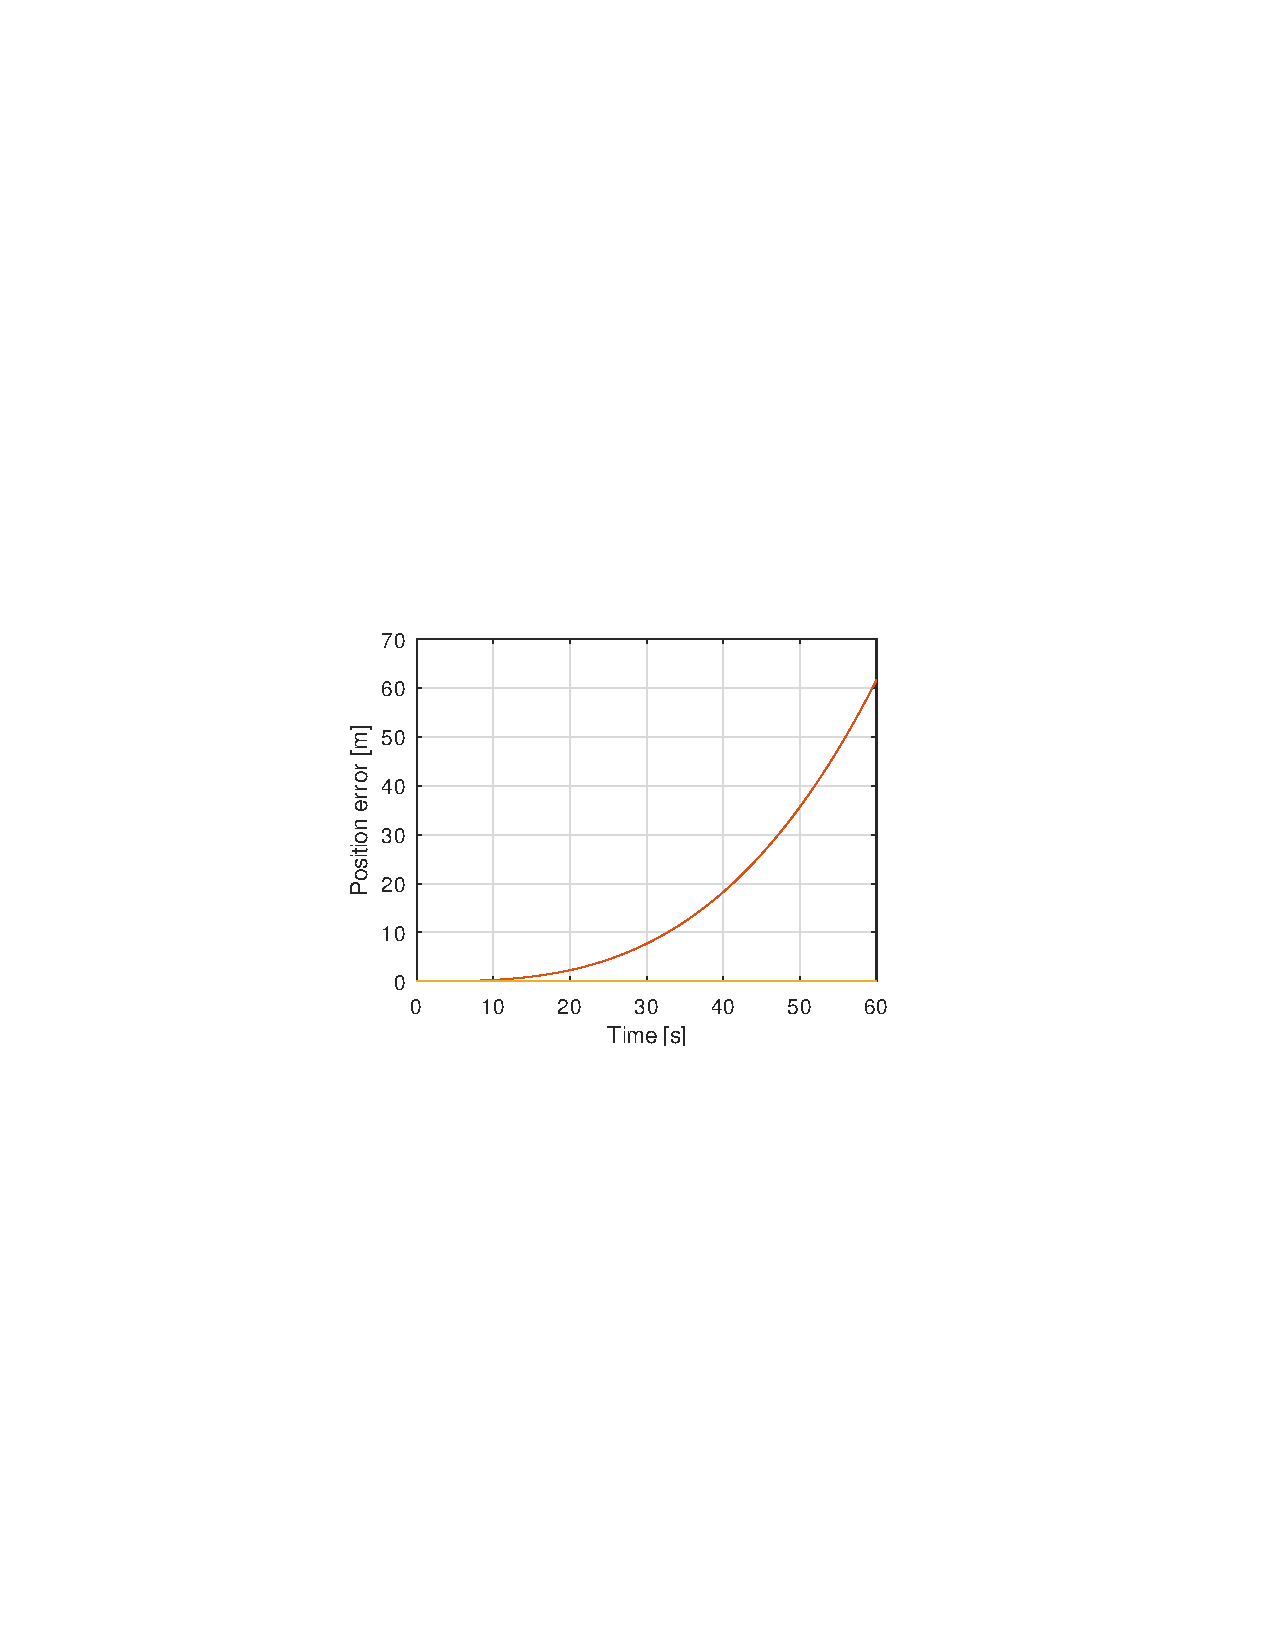
\includegraphics[]{images/error_growth.pdf}
    \caption{Acceleration vs. Time When dropped from the 2nd floor.}
    \label{fig:my_label}
\end{figure}
\end{frame}

% \begin{frame}
% \frametitle{References}

% \setbeamertemplate{bibliography item}[text]

% \bibliographystyle{acm}
% \bibliography{mobility.bib}
% \end{frame}
\end{document}
